%#Split: 01_background  
%#PieceName: p01_background
% p01_background_00.tex
\KLBeginSubjectWithHeaderCommands{01}{2}{研究の位置づけ}{1}{F}{3}{\DCPDVeryFirstPageStyle}{\DCPDDefaultPageStyle}

\section{研究の位置づけ}
%    <<最大 1ページ>>

%s03_background
本研究は、フェイクニュースの早期自動検出に向け、ユーザからの情報提供の活用を目指すものである。

%begin 背景: 当該分野の状況 ====================
\graysubsection{当該分野の状況: フェイクニュースの自動検出}

\setlength\intextsep{0pt}
\setlength\textfloatsep{0pt}
\begin{wrapfigure}{r}[10pt]{0.3\linewidth}
%    \vspace{-5mm}
    \centering
    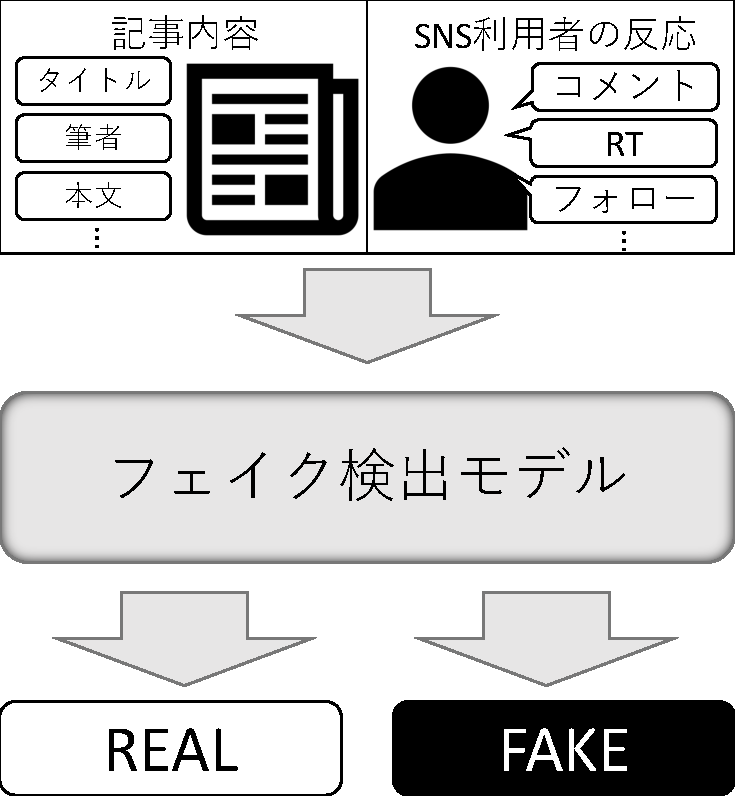
\includegraphics[width=0.3\textwidth]{figs/base_model.pdf}
    \vspace{-1cm} 
    \caption{フェイクニュース自動検出の基本的な流れ}
    \label{fig:objects}
\end{wrapfigure}
SNSの発展で情報を迅速かつ大量に取得・共有が容易になった一方、
悪意により他人を騙すために作られた\textbf{フェイクニュース}も拡散されやすくなった。
特に2020年からCOVID-19の影響による誤情報の拡散であるインフォデミックにより、
メタノール飲用による死亡事故\cite{iraninfo}といった事象が報告された。
以上から騙された人々の命に関わる被害が起きるため、
\underline{フェイクニュース拡散の早期抑制が必要である}\cite{snsinfo}。

フェイクニュースの検出方法として有識者が記事内容を調査する\textbf{ファクトチェック}があるが、
拡散ののち着手されるため\underline{拡散抑制にはならない}。
そのため自動でフェイクニュースを検出するべく、
図\ref{fig:objects}のようにファクトチェック結果をラベルとして、記事内容や利用者の反応から教師あり深層学習で自動検出する研究がある\cite{Wang:2018:EEA:3219819.3219903}。
%end 背景: 当該分野の状況 ====================

%begin 背景: 課題 ====================
\graysubsection{課題}
フェイクニュース自動検出が抱える課題は以下の通りである。
\vspace{-3mm}
\begin{description}
    %\vspace{-5mm}
    \setlength{\parskip}{0cm}
    \setlength{\itemsep}{0cm}
    \item[分野や出来事による特異性] %\mbox{}\\
        ニュースという性質上、フェイクニュースで扱われる分野や出来事で内容が異なるため対応を難しくしている。
        先行研究によると学習・検証で入力するニュースの出来事を変えると検出性能が劣化する\cite{Wang:2018:EEA:3219819.3219903}。
        よって分野や出来事に左右されない\underline{普遍的な検出モデルが必要}である。
%    \item[SNSプラットフォームへの依存性] %\mbox{}\\
%        SNS上で利用者からの反応を取得する場合、その形式は取得元のSNSプラットフォームに依存する。
%        今後主流となるSNSが変わった場合、利用者層や時代の違いにより\underline{既存のデータでは対応できない}。
    \item[早期検出と正確性の両立] %\mbox{}\\
        記事内容に加えて利用者の反応(RT, コメント等)を扱うと検出性能が改善する\cite{Wu:2018:TFF:3159652.3159677}一方、
        利用者の反応を十分に得るには時間がかかり、\underline{高い正確性と早期検出を両立できない}。
        利用者に反応を示すよう自動的に促進する方法はbotによる拡散等が挙げられる一方、フェイクニュース拡散も促進するリスクも伴う。
    \item[日本語データセット不足] %\mbox{}\\
        深層学習による検出は、正解ラベルとして多量のファクトチェック結果を要する。
        このファクトチェックが活発な地域差の影響でデータセットが英語に集中\cite{fakenewsnet}している。
        もし日本語を対象とした場合、ラベル不足の影響により\underline{教師あり学習ができない}。
        この影響により言語を問わない検出を視野に入れた研究も難しくしている。
    \end{description}
%end 背景: 課題 ====================

%begin 着想に至った経緯 ====================
\graysubsection{本研究計画の着想に至った経緯}
私は修士課程で\underline{英文フェイクニュース早期検出の研究を行った}。
記事へのコメントが検出に有用とする先行研究\cite{defend}をベースに、
早期検出を想定し限られた\underline{少量コメントから自動でコメントを追加で生成}してから記事の真偽判断する手法を実装した。
実験にて提案手法がより多くのフェイクニュースを検出した(p.7, 成果\ref{enum:ines}: \cite{ines})
が、時に判断に不要なコメントが生成された場合は誤判断を誘発していた。
%コメントの自動生成のみでは利用者に対し有用な判断理由を得るには難しい点に直面したため、
それゆえSNS利用者から\underline{真偽判断において重要な情報である手がかり}を得る重要性に着目した。

また社会変化で
%ユーザの反応を多く使うことが難しい早期検出の実現への難しさに加えて、
主流のニューストピックと同時にフェイクニュースの内容も変わるため、
%利用者の反応が現れるSNSプラットフォームも近年は新しいサービスが提供されている。
%この影響でこれまでの記事+SNS上の反応を扱う検出形式では、
データセット・モデル提供と拡張の仕組みのみでは\underline{時代の変化に対応できない}。
一方、一般論としてトピックや言語に問わずフェイクと強く疑われる記事の特徴は一致しているため、
\underline{普遍的な特徴から検出するモデルの開発}にも着目した。
%一方、国内研究会で発表したところ想定以上に日本語での実現に対する期待を受けた。
%日本は英語圏に比べファクトチェックされた記事が少なく、
%\underline{データセットを作ってモデルを実装するにはラベルが足りない}。
%このラベル不足を補う方法として、少量のラベル付き記事と多量のラベルなし記事に利用者の初期反応から
%弱いアノテーションを付加して学習を行う弱教師あり学習を行う研究\cite{mwss}に着目した。
%日本語で同じ構成のデータセットを作成し、分類を行うモデルを実装することで実現可能と考えた。

%end 着想に至った経緯 ====================

{\footnotesize 
%\vspace{1cm}
\begin{twobibliography}{99}
    \setlength{\parskip}{0cm}
    \setlength{\itemsep}{0cm}
    \bibitem{iraninfo} H. Hassanian-Moghaddam, \textit{et al.} \textit{Critical Care} 24.1 2020: 1-3.
    \bibitem{snsinfo} S. Tasnim, \textit{et al.} \textit{JPMPH} 53.3 2020: 171-174.
    \bibitem{Wang:2018:EEA:3219819.3219903} Y. Wang, \textit{et al.} \textit{KDD'18}, pp. 849-857. 2018.
    \bibitem{Wu:2018:TFF:3159652.3159677} L. Wu \& H. Liu. \textit{WSDM '18}  pp. 637-645, 2018.
    \bibitem{fakenewsnet} K. Shu,\textit{et al.} \textit{Big Data 8.3} 2020: 171-188.
    \bibitem{coviddiff} Y. Bang, \textit{et al.} \textit{arXiv preprint arXiv:2101.03841} 2021.
    \bibitem{defend} K. Shu, \textit{et al.} \textit{KDD'19} 395–405, 2019.
    \bibitem{ines} Y. Yanagi, \textit{et al.} \textit{INES}. 2020.
    \bibitem{mwss} K. Shu, \textit{et al.}  \textit{arXiv preprint arXiv:2004.01732} 2020.
\end{twobibliography}
}
% p01_background_01.tex
\KLEndSubject{F}


